% Archivo generado automaticamente por scripts/procesar_resultados.py
\section{Resultados autom\'aticos de pruebas}
\label{sec:resultados-automaticos}
\subsection{Prueba1}
\begin{table}[h]
\centering
\begin{tabular}{l c c c c c c c}
\toprule
Sesion & Nodos & Lat (ms) & P\'erdida (\%) & msg/s & Mbps & RSSI (dBm) & TX/RX Mbps\\
\midrule
Prueba1_20251203-014820-s00000-n00020 & 20 & 10.342 & 0.000 & 1.847 & 0.002 & - & -/-\\
\bottomrule
\end{tabular}
\caption{Resumen del escenario Prueba1.}
\end{table}
\begin{figure}[h]
\centering
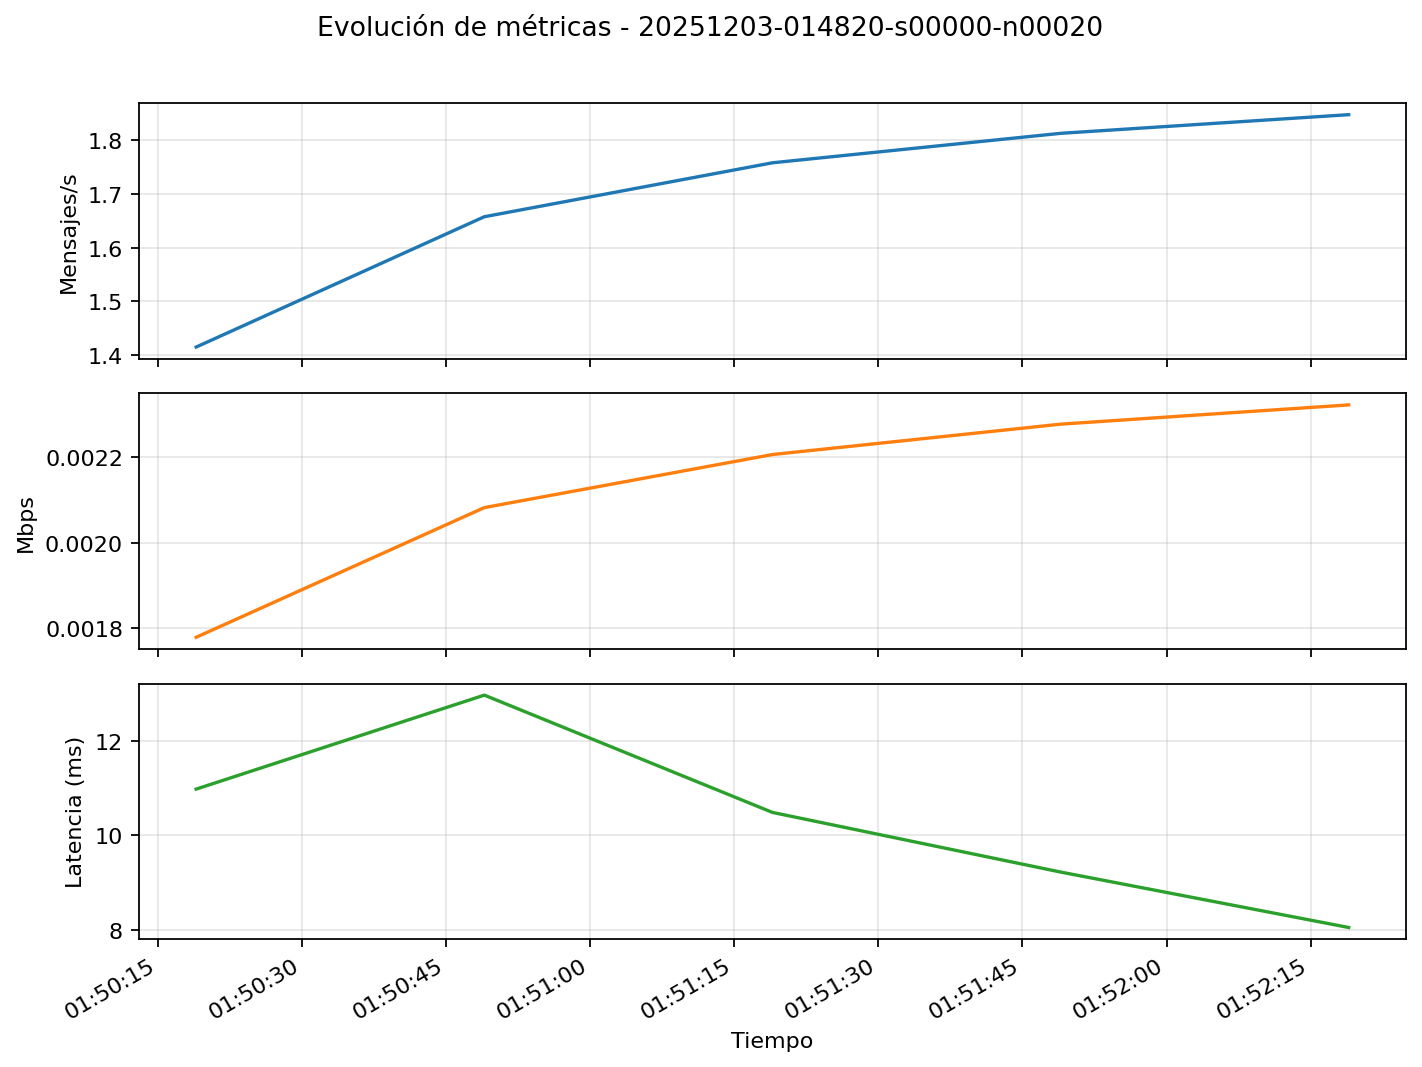
\includegraphics[width=0.9\linewidth]{data/metrics/reports/Prueba1_20251203-014820-s00000-n00020-overview.png}
\caption{M\'etricas para Prueba1 (Prueba1_20251203-014820-s00000-n00020).}
\end{figure}
\paragraph{Conclusiones autom\'aticas}
\begin{itemize}
  \item Se ejercitaron aproximadamente 20 dispositivos.
  \item La entrega fue estable con pérdida <1%.
  \item La latencia promedio se mantuvo baja para el escenario evaluado.
  \item El throughput pico fue cercano a 1.85 msg/s.
\end{itemize}
\subsection{Prueba2_n50}
\begin{table}[h]
\centering
\begin{tabular}{l c c c c c c c}
\toprule
Sesion & Nodos & Lat (ms) & P\'erdida (\%) & msg/s & Mbps & RSSI (dBm) & TX/RX Mbps\\
\midrule
Prueba2_n50_20251203-220654-s00000-n00050 & 50 & 5.810 & 64.454 & 7.909 & 0.010 & - & -/-\\
Prueba2_n50_20251203-221853-s00000-n00050 & 50 & 3.658 & 0.000 & 9.358 & 0.012 & - & -/-\\
\bottomrule
\end{tabular}
\caption{Resumen del escenario Prueba2_n50.}
\end{table}
\begin{figure}[h]
\centering
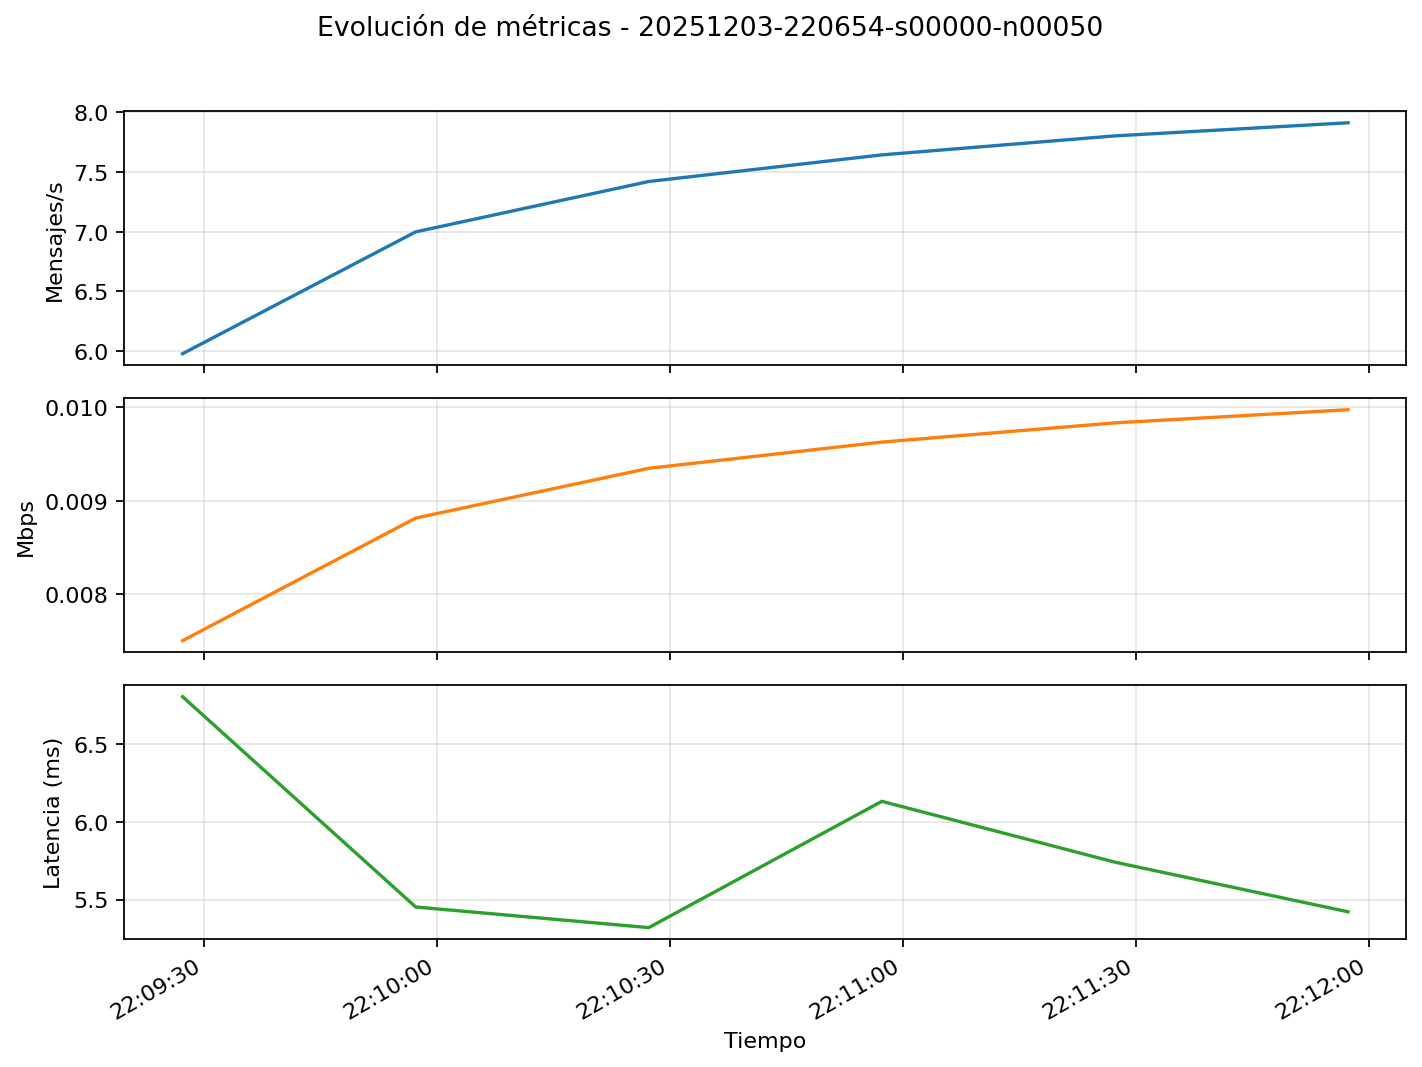
\includegraphics[width=0.9\linewidth]{data/metrics/reports/Prueba2_n50_20251203-220654-s00000-n00050-overview.png}
\caption{M\'etricas para Prueba2_n50 (Prueba2_n50_20251203-220654-s00000-n00050).}
\end{figure}
\begin{figure}[h]
\centering
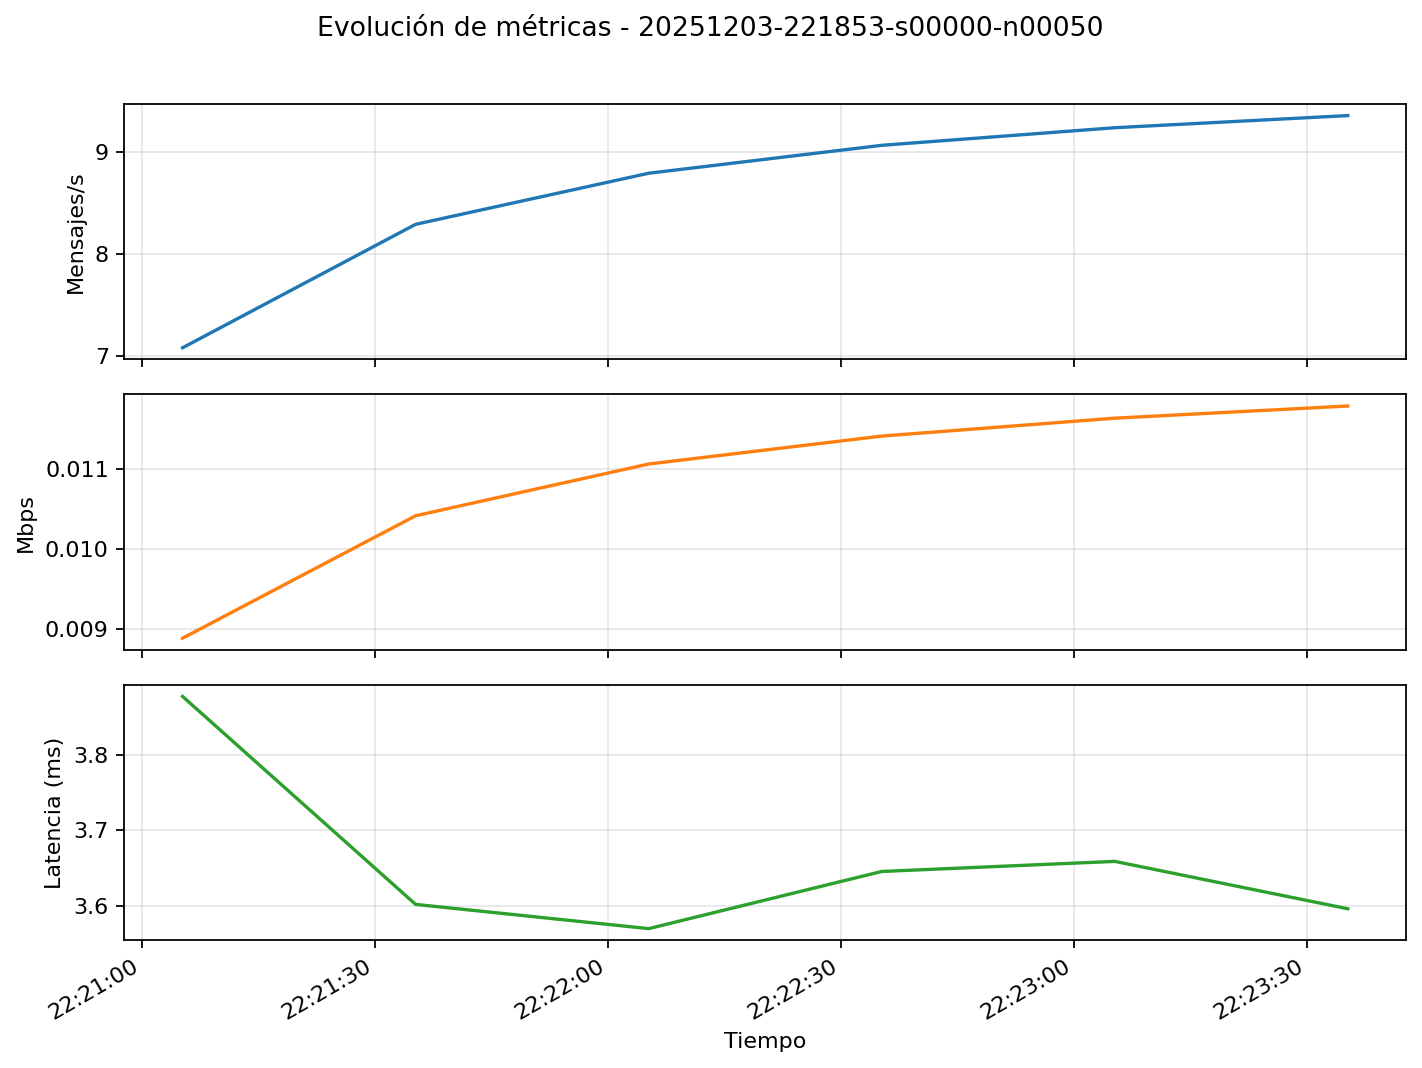
\includegraphics[width=0.9\linewidth]{data/metrics/reports/Prueba2_n50_20251203-221853-s00000-n00050-overview.png}
\caption{M\'etricas para Prueba2_n50 (Prueba2_n50_20251203-221853-s00000-n00050).}
\end{figure}
\paragraph{Conclusiones autom\'aticas}
\begin{itemize}
  \item Se ejercitaron aproximadamente 50 dispositivos.
  \item La entrega fue estable con pérdida <1%.
  \item La latencia promedio se mantuvo baja para el escenario evaluado.
  \item El throughput pico fue cercano a 9.36 msg/s.
\end{itemize}
\subsection{Prueba2_n100}
\begin{table}[h]
\centering
\begin{tabular}{l c c c c c c c}
\toprule
Sesion & Nodos & Lat (ms) & P\'erdida (\%) & msg/s & Mbps & RSSI (dBm) & TX/RX Mbps\\
\midrule
Prueba2_n100_20251203-222418-s00000-n00100 & 100 & 5.756 & 0.000 & 18.721 & 0.024 & - & -/-\\
\bottomrule
\end{tabular}
\caption{Resumen del escenario Prueba2_n100.}
\end{table}
\begin{figure}[h]
\centering
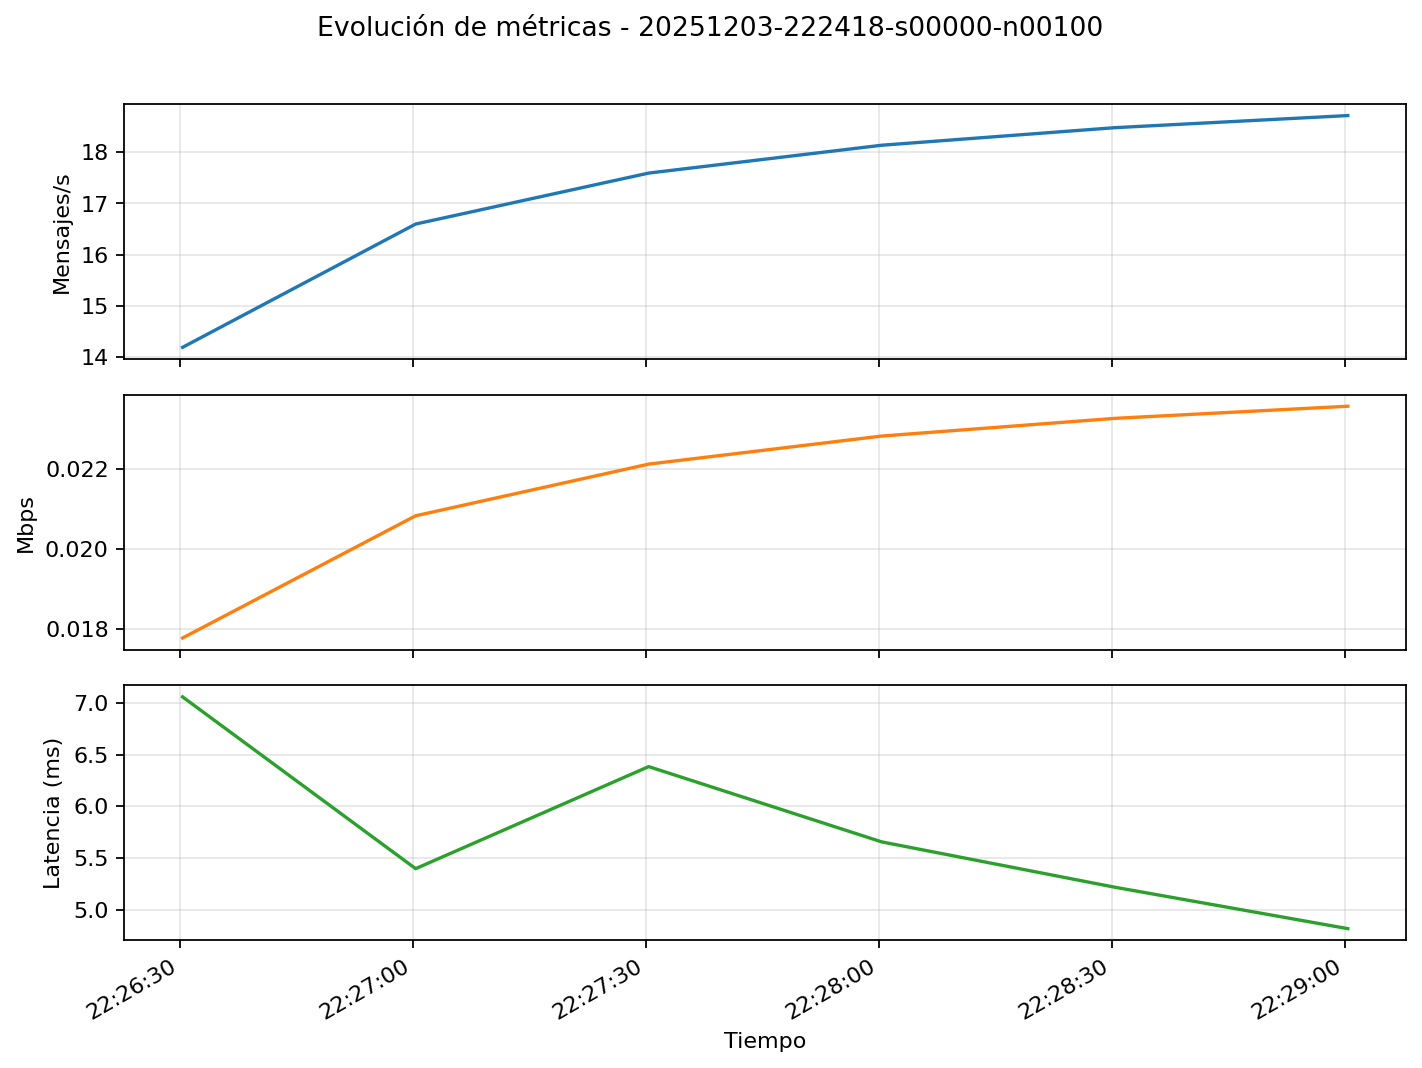
\includegraphics[width=0.9\linewidth]{data/metrics/reports/Prueba2_n100_20251203-222418-s00000-n00100-overview.png}
\caption{M\'etricas para Prueba2_n100 (Prueba2_n100_20251203-222418-s00000-n00100).}
\end{figure}
\paragraph{Conclusiones autom\'aticas}
\begin{itemize}
  \item Se ejercitaron aproximadamente 100 dispositivos.
  \item La entrega fue estable con pérdida <1%.
  \item La latencia promedio se mantuvo baja para el escenario evaluado.
  \item El throughput pico fue cercano a 18.72 msg/s.
\end{itemize}
\subsection{Prueba3_int10}
\begin{table}[h]
\centering
\begin{tabular}{l c c c c c c c}
\toprule
Sesion & Nodos & Lat (ms) & P\'erdida (\%) & msg/s & Mbps & RSSI (dBm) & TX/RX Mbps\\
\midrule
Prueba3_int10_20251203-225401-s00000-n00200 & 200 & 9.288 & 0.000 & 18.720 & 0.024 & - & -/-\\
\bottomrule
\end{tabular}
\caption{Resumen del escenario Prueba3_int10.}
\end{table}
\begin{figure}[h]
\centering
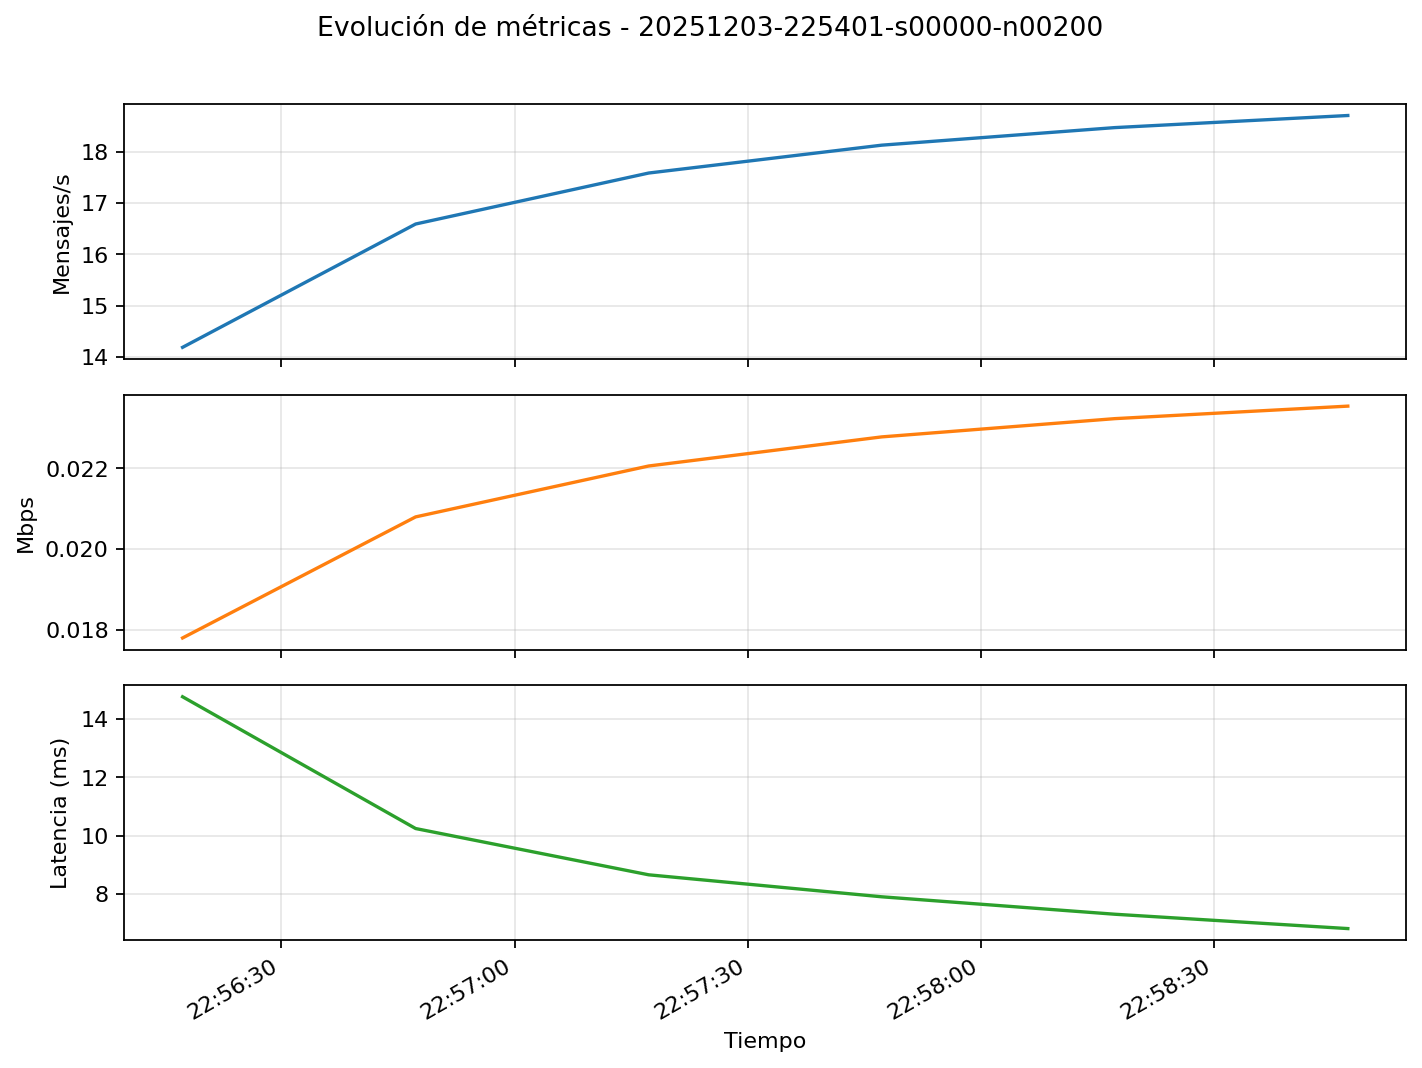
\includegraphics[width=0.9\linewidth]{data/metrics/reports/Prueba3_int10_20251203-225401-s00000-n00200-overview.png}
\caption{M\'etricas para Prueba3_int10 (Prueba3_int10_20251203-225401-s00000-n00200).}
\end{figure}
\paragraph{Conclusiones autom\'aticas}
\begin{itemize}
  \item Se ejercitaron aproximadamente 200 dispositivos.
  \item La entrega fue estable con pérdida <1%.
  \item La latencia promedio se mantuvo baja para el escenario evaluado.
  \item El throughput pico fue cercano a 18.72 msg/s.
\end{itemize}
